\documentclass[12pt,a4paper]{article}
\usepackage[utf8]{inputenc}
\usepackage{amsmath, amsthm, amssymb, amsfonts}
\usepackage{mathtools}
\usepackage{graphicx}
\usepackage[T1]{fontenc}
\usepackage[absolute,overlay]{textpos}
\usepackage{braket}  % bra-ket notation
\usepackage{slashed} % Dirac notation
\usepackage{tikz-feynman,contour}
\usepackage{breqn}   % Equation breaking
\usepackage{mathptmx}
\usepackage{fullpage}
\usepackage{units}

%\usepackage[printwatermark]{xwatermark}
%\newwatermark[allpages,color=black!20,angle=45,scale=2,xpos=0,ypos=0]{WORK IN PROGRESS}

\usepackage{hyperref}
\hypersetup{
    colorlinks,
    citecolor=blue,
    filecolor=black,
    linkcolor=black,
    urlcolor=black
}

\author{Robert Kralik}
\title{Theoretical overview for the neutrino magnetic moment analysis}

%\linenumbers % Include line numbers

\begin{document}
\maketitle
\tableofcontents
\newpage

\section{Electromagnetic properties of the neutrino}

%In the Standard Model (SM) neutrinos are electrically neutral and do not interact with photons at the tree level. However, radiative corrections generate neutrino interactions with photons through loops involving the charged leptons and the W boson, as shown by the one-loop diagrams in Fig. 9(a). The corresponding neutrino-photon interactions are described by charge radii of the flavor neutrinos . Therefore, even in the SM, where neutrinos are neutral and massless, there are non-zero neutrino electromagnetic properties. [NeutrinoPropertiesSnowmass2022.pdf]

% Although in the standard model neutrinos are electrically neutral and do not possess electric or magnetic dipole moments, they have a charge radius which is generated by radiative corrections. [...] In many extensions of the standard model neutrinos also acquire electromagnetic properties through quantum loop effects which allow direct interactions of neutrinos with electromagnetic fields and electromagnetic interactions of neutrinos with charged particles. Hence, the theoretical and experimental study of neutrino electromagnetic interactions is a powerful tool in the search for the fundamental theory beyond the standard model. Moreover, the electromagnetic interactions of neutrinos can generate important effects, especially in astrophysical environments, where neutrinos propagate over long distances in magnetic fields in vacuum and in matter. [nuElmagInt2015.pdf]

% ...the existence of neutrino masses and mixing implies that neutrinos have magnetic moments. Since their values depend on the specific theory which extends the standard model in order to accommodate neutrino masses and mixing, experimentalists and theorists are eagerly looking for them. [nuElmagInt2015.pdf]

In the standard model, neutrino can have electromagnetic interaction only at a higher order of the perturbative expansion of the interaction - from loop diagrams. In the one photon approximation, the electromagnetic interactions of a neutrino field $\left(\nu_k\left(x\right), k\in\left\lbrace 1,...,N\right\rbrace\right)$, for $N$ neutrino mass states, can be described by the effective interaction Hamiltonian \cite{nuElmagInt2015.pdf}
\begin{equation}
\mathcal{H}^{\left(\nu\right)}_{em}\left(x\right)=\sum^N_{k,j=1}\overline{\nu}_k\left(x\right)\Lambda^{kj}_{\mu}\nu_j\left(x\right)A^{\mu}\left(x\right)
\end{equation}
and the amplitude of neutrino-to-neutrino interaction for \textbf{Dirac} neutrinos shown on fig.\ref{figFeynman} is
\begin{equation}
\braket{\nu_f\left(p_f\right)|j^{\left(\nu\right)}_{\mu}\left(x\right)|\nu_i\left(p_i\right)}=
e^{i\left(p_f-p_i\right)x}\overline{u}_f\left(p_f\right)\Lambda^{fi}_{\mu}\left(p_f,p_i\right)u_i\left(p_i\right),
\end{equation}
where $p_f$ and $p_i$ are the final and initial four momentums respectively and $u/\overline{u}$ are the solutions to the Dirac equation for a free particle. We take into account possible transitions between different mass states $\nu_i$ and $\nu_f$ \cite{nuElmagInt2015.pdf}.

\begin{figure}
\centering
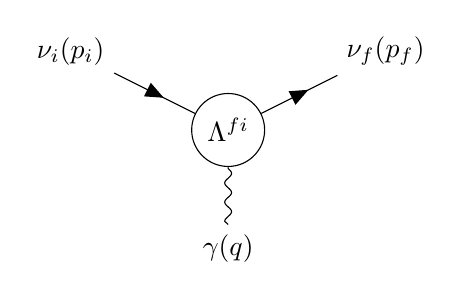
\begin{tikzpicture}
  \begin{feynman}
    \vertex[draw,circle] (m) at ( 0, 0) {$\Lambda^{fi}$};
    \vertex (a) at (-2,1) {\(\nu_i(p_i)\)};
    \vertex (b) at (2,1) {\(\nu_f(p_f)\)};
    \vertex (c) at (0,-1.5) {\(\gamma(q)\)};

    \diagram* {
      (a) -- [fermion] (m) -- [fermion] (b),
      (m) -- [boson] (c)
    };
  \end{feynman}
\end{tikzpicture}
\caption{Effective coupling of neutrinos with one photon electromagnetic field.}
\label{figFeynman}
\end{figure}

The vertex function $\Lambda^{fi}_{\mu}\left(p_f,p_i\right)$ is a matrix and in the most general case it can be written in terms of linearly independent products of Dirac matrices $\left(\gamma\right)$ and four momentum of the photon $\left(q=p_f-p_i\right)$:
\begin{align}
\Lambda^{fi}_{\mu}\left(p_f,p_i\right)=&
\mathbb{F}^{fi}_1\left(q^2\right)q_{\mu}+
\mathbb{F}^{fi}_2\left(q^2\right)q_{\mu}\gamma_5+
\mathbb{F}^{fi}_3\left(q^2\right)\gamma_{\mu}+
\mathbb{F}^{fi}_4\left(q^2\right)\gamma_{\mu}\gamma_5+\notag\\ &
\mathbb{F}^{fi}_5\left(q^2\right)\sigma_{\mu\nu}q^{\nu}+
\mathbb{F}^{fi}_6\left(q^2\right)\epsilon_{\mu\nu\rho\gamma}q^{\nu}\sigma^{\rho\gamma},
\end{align}
where $\mathbb{F}^{fi}_i\left(q^2\right)$ are six Lorentz invariant form factors. For $f=i$ they are called "diagonal" and for $f\neq i$ "transition form factors" \cite{nuElmagInt2015.pdf}.

Applying conditions of hermiticity $\left(\mathcal{H}^{\left(\nu\right)\dagger}_{em}=\mathcal{H}^{\left(\nu\right)}_{em}\right)$ and of conservation of the current (continuity equation: 
$\partial^{\mu}j^{\left(\nu\right)}_{\mu}\left(x\right)=0$), we can rewrite the vertex function as
\begin{equation}
\Lambda^{fi}_{\mu}\left(q\right)=
\left(\gamma_{\mu}-q_{\mu}\slashed{q}/q^2\right)\left[
\mathbb{F}^{fi}_{Q}\left(q^2\right)+\mathbb{F}^{fi}_{A}\left(q^2\right)q^2\gamma_5\right]-
i\sigma_{\mu\nu}q^{\nu}\left[\mathbb{F}^{fi}_{M}\left(q^2\right)+i\mathbb{F}^{fi}_{E}\left(q^2\right)\gamma_5\right],
\end{equation}
where $\mathbb{F}^{fi}_Q,\mathbb{F}^{fi}_M,\mathbb{F}^{fi}_E$ and $\mathbb{F}^{fi}_A$ are hermitian matrices representing the real charge, dipole magnetic, dipole electric and anapole neutrino form factors. In coupling with a real photon $\left(q^2=0\right)$ these become the neutrino charge, magnetic, electric and anapole moment \cite{nuElmagInt2015.pdf}.

For antineutrinos the form factors are transformed as:
\begin{equation}\label{eqAnu1}
\overline{\mathbb{F}}^{fi}_{\Omega}=-\mathbb{F}^{if}_{\Omega}=-\left(\mathbb{F}^{fi}_{\Omega}\right)^{\star} \ \ \ \Omega=Q,M,E,
\end{equation}
\begin{equation}\label{eqAnu2}
\overline{\mathbb{F}}^{fi}_{A}=\mathbb{F}^{if}_{A}=\left(\mathbb{F}^{fi}_{A}\right)^{\star}.
\end{equation}

In case of \textbf{Majorana neutrinos}, the general expression for the vertex function in terms of charge, magnetic, electric and anapole form factors looks the same as for Dirac neutrinos. However, since Majorana antineutrinos are the same particle as Majorana neutrinos, from eq.\ref{eqAnu1},\ref{eqAnu2} we can see that:
\begin{equation}\label{eqAntisymmetryCondition}
\mathbb{F}^M_{\Omega}=-\left(\mathbb{F}^M_{\Omega}\right)^T \ \ \ \Omega=Q,M,E,
\end{equation}
\begin{equation}
\mathbb{F}^M_{A}=\left(\mathbb{F}^M_A\right)^T.
\end{equation}
Therefore the Majorana charge, magnetic and electric form factor matrices are antisymmetric and the anapole form factor matrix is symmetric. This means that Majorana neutrino doesn't have any diagonal charge and dipole magnetic and electric moments, but it can have transition  charge and magnetic and electric moment \cite{nuElmagInt2015.pdf}.

%%%%%%%%%%%%%%%%%%%%%%%%%%%%%%%%%%%%%%%%
\section{Neutrino electric and magnetic dipole moments}

Evaluating the one loop diagrams in the minimal extension of the standard model with right handed (Dirac) neutrinos gives us the first approximation of the electric and magnetic moments $\left(q^2=0\right)$:
\begin{equation}
\begin{rcases}
\mu^D_{kj}\\
i\epsilon^D_{kj}
\end{rcases}
\simeq\frac{3eG_F}{16\sqrt{2}\pi^2}\left(m_k\pm m_j\right)\left(\delta_{kj}-\frac{1}{2}\sum_{l=e,\mu ,\tau}U^{\star}_{lk}U_{lj}\frac{m_l^2}{m_W^2}\right),
\end{equation}
where $m_k,m_j$ are the neutrino masses, but $m_l$ are the masses of charged leptons which appear in the loop diagrams. Higher order electromagnetic corrections were neglected, but those can also have a significant contribution \cite{nuElmagInt2015.pdf}.

There are no diagonal electric moments $\left(\epsilon_{kk}^D=0\right)$ and the diagonal magnetic moments are approximately
\begin{equation}\label{DiagMagMomVal}
\mu_{kk}^D\simeq\frac{3eG_Fm_k}{8\sqrt{2}\pi^2}\simeq 3.2\times 10^{-19}\left(\frac{m_k}{\textsf{eV}}\right)\mu_B,
\end{equation}
where $\mu_B$ is the Bohr magneton \cite{nuElmagInt2015.pdf}.

The transition magnetic moments are suppressed with respect to the largest of the diagonal magnetic moments by at least a factor of $10^{-4}$ due to the $m_W^2$ in denominator and the transition electric moments are even smaller than that due to the mass difference \cite{nuElmagInt2015.pdf}. Therefore an experimental observation of a magnetic moment larger than in eq.\ref{DiagMagMomVal} would indicate physics beyond the minimally extended standard model \cite{nuMMMajoranaBounds2006.pdf}.

Majorana neutrinos can be obtained by either adding a $\textsf{SU}\left(2\right)_L$ Higgs triplet, or right handed neutrinos together with a $\textsf{SU}\left(2\right)_L$ Higgs singlet. If we neglect the Feynman diagrams which depend on the model of the scalar sector, the magnetic and electric dipole moments are
\begin{equation}
\mu_{kj}^M\simeq -\frac{3ieG_F}{16\sqrt{2}\pi^2}\left(m_k+m_j\right)\sum_{l=e,\mu ,\tau}\operatorname{Im}\left[U^{\star}_{lk}U_{lj}\right]\frac{m_l^2}{m_W^2},
\end{equation}
\begin{equation}
\epsilon_{kj}^M\simeq \frac{3ieG_F}{16\sqrt{2}\pi^2}\left(m_k-m_j\right)\sum_{l=e,\mu ,\tau}\operatorname{Re}\left[U^{\star}_{lk}U_{lj}\right]\frac{m_l^2}{m_W^2}.
\end{equation}
These are difficult to compare to the Dirac case, due to possible presence of Majorana phases in the PMNS matrices, but it is clear that they have the same order of magnitude as Dirac transition dipole moments. However, the neglected model dependent contributions can enhance the transition dipole moments \cite{nuElmagInt2015.pdf}.

It is possible \cite{nuMMMajoranaBounds2006.pdf} to obtain "natural" upper limits on the size of neutrino magnetic moment by calculating its contribution to the neutrino mass by standard model radiative corrections. For Dirac neutrinos the radiative correction induced by neutrino magnetic moment, generated at an energy scale $\Lambda$, to the neutrino mass is generically
\begin{equation}
m_{\nu}^D\sim\frac{\mu_{\nu}^D}{3\times 10^{-15}\mu_B}\left[\Lambda\left(\textsf{TeV}\right)\right]^2\textsf{eV}.
\end{equation}
So for $\Lambda\simeq 1\textsf{TeV}$ and $m_{\nu}\lesssim 0.3\textsf{eV}$ the limit becomes $\mu_{\nu}^D\lesssim 10^{-15}\mu_B$. This applies only if the new physics is well above the electroweak scale ($\Lambda_{EW} \sim 100\textsf{GeV}$). It is possible to get Dirac neutrino magnetic moment higher than this limit, for example in frameworks of minimal super-symmetric standard model, by adding more Higgs doublets, or by considering large extra dimensions \cite{nuElmagInt2015.pdf}.

The limit for Majorana neutrino magnetic moment is less stringent, due to the antisymmetry condition from eq.\ref{eqAntisymmetryCondition} and considering $m_{\nu}\lesssim 0.3\textsf{eV}$ can be expressed as
\begin{align}
\mu_{\tau\mu},\mu_{\tau e} &\lesssim 10^{-9}\left[\Lambda\left(\textsf{TeV}\right)\right]^{-2}\\
\mu_{\mu e} &\lesssim 3\times 10^{-7}\left[\Lambda\left(\textsf{TeV}\right)\right]^{-2}
\end{align}
which is shown in the flavour basis , which relates to the framework used previously as
\begin{equation}
\mu_{ij}=\sum_{\alpha\beta}\mu_{\alpha\beta}U^{\star}_{\alpha i}U_{\beta j},\ \ \ \alpha,\beta\in\left\lbrace e,\mu,\tau\right\rbrace.
\end{equation}
This limits imply, that if a magnetic moment $\mu\gtrsim 10^{-15}\mu_B$ would be measured, it is plausible neutrinos are Majorana fermions and the scale of lepton violation would be well below the conventional see-saw scale \cite{nuMMMajoranaBounds2006.pdf}.

%%%%%%%%%%%%%%%%%%%%%%%%%%%%%%%%%%%%%%%%%%%%%%%%

\section{Measuring neutrino magnetic moment}
\subsection{Effective neutrino magnetic moment}
What we measure in experiments is an effective "flavour" magnetic moment, which is influenced by mixing of "mass" magnetic moments (and electric moments) and oscillations. In the ultrarelativistic limit this is
\begin{equation}
\mu_{\nu_l}^2\left(L,E_{\nu}\right)=\sum_j\left|\sum_k U^{\star}_{lk}e^{-i\Delta m^2_{kj}L/2E_{\nu}}\left(\mu_{jk}-i\epsilon_{jk}\right)\right|^2.
\end{equation}
What is called the effective magnetic moment (often just magnetic moment) therefore contains contributions from both the neutrino magnetic and electric moment \cite{nuElmagInt2015.pdf}.

For antineutrinos, the effective magnetic moment is
\begin{equation}
\mu_{\overline{\nu}_l}^2\left(L,E_{\nu}\right)=\sum_j\left|\sum_k U^{\star}_{lk}e^{+i\Delta m^2_{kj}L/2E_{\nu}}\left(\mu_{jk}-i\epsilon_{jk}\right)\right|^2.
\end{equation}
So the only difference is in the phase induced by neutrino oscillations.

For experiments with baselines short enough for neutrino oscillations to not develop ($\frac{\Delta m^2L}{2E_{\nu}}\ll~1$), such as the NOvA ND, the effective magnetic moment can be expressed as
\begin{equation}
\mu_{\nu_l}^2\simeq\mu_{\overline{\nu}_l}^2\simeq\sum_j\left|\sum_k U_{lk}^{\star}\left(\mu_{jk}-i\epsilon_{jk}\right)\right|^2=\left[U\left(\mu^2+\epsilon^2\right)U^{\dagger}+2\operatorname{Im}\left(U\mu\epsilon U^{\dagger}\right)\right]_{ll^{\prime}},
\end{equation}
which is independent of the neutrino energy and of the source to detector distance.

It is important to mention, that since the effective magnetic moment depends on the flavour of the studied neutrino, it is different for different types of neutrino experiment. Also the solar neutrino experiments need to include the effect of the solar matter on the neutrino oscillations. Therefore the reports on the value (or upper limit) of the effective neutrino magnetic moment are not directly comparable between different types of neutrino experiments.

\subsection{Neutrino-on-electron elastic scattering}
The most sensitive method to measure neutrino magnetic moment is the low energy elastic scattering of (anti)neutrinos on electrons \cite{nuElmagInt2015.pdf}. This interaction has two observables, the recoil electron's kinetic energy $\left(T_e\right)$ and the recoil angle with respect to the incoming neutrino beam $\left(\theta\right)$. From simple $2\rightarrow 2$ kinematics we can get
\begin{equation}
\left(P_{\nu}-P_{e^{\prime}}\right)^2=\left(P_{\nu^{\prime}}-P_e\right)^2,
\end{equation}
\begin{equation}
m_{\nu}^2+m_e^2-2E_{\nu}E_{e^{\prime}}+2E_{\nu}p_{e^{\prime}}\cos\theta=m_{\nu}^2+m_e^2-2E_{\nu^{\prime}}m_e.
\end{equation}
Using the energy conservation
\begin{equation}
E_{\nu}+m_e=E_{\nu^{\prime}}+E_{e^{\prime}}=E_{\nu^{\prime}}+T_e+m_e\Rightarrow E_{\nu^{\prime}}=E_{\nu}-T_e
\end{equation}
we get
\begin{equation}
E_{\nu}p_{e^{\prime}}\cos\theta=E_{\nu}E_{e^{\prime}}-E_{\nu^{\prime}}m_e=E_{\nu}\left(T_e+m_e\right)-\left(E_{\nu}-T_e\right)m_e=T_e\left(E_{\nu}+m_e\right),
\end{equation}
\begin{equation}
\cos\theta=\frac{E_{\nu}+m_e}{E_{\nu}}\sqrt{\frac{T_e^2}{E_{e^{\prime}}^2-m_e^2}}=\frac{E_{\nu}+m_e}{E_{\nu}}\sqrt{\frac{T_e^2}{T_e^2+2T_em_e}}.
\end{equation}
And finally we get
\begin{equation}\label{eqThetaTRelation}
\cos\theta=\frac{E_{\nu}+m_e}{E_{\nu}}\sqrt{\frac{T_e}{T_e+2m_e}}.
\end{equation}
Electron's kinetic energy is kinematically constrained by
\begin{equation}
T_e\leq\frac{2E_{\nu}^2}{2E_{\nu}+m_e}.
\end{equation}

Considering $E_{\nu}\sim\textsf{GeV}$, we can approximate $\frac{m_e^2}{E_{\nu}^2}\rightarrow 0$ and in the small angle approximation we get from eq.\ref{eqThetaTRelation} 
\begin{equation}\label{eqTThetaSqExp}
T\theta^2\cong 2m_e\left(1-\frac{T_e}{E_{\nu}}\right)<2m_e.
\end{equation}

In the ultrarelativistic limit, the neutrino magnetic moment changes the neutrino helicity, turning active neutrinos into sterile. Since the SM weak interaction conserves helicity we can add the two contribution to the neutrino on electron cross section incoherently \cite{nuElmagInt2015.pdf}:
\begin{equation}
\frac{d\sigma_{\nu_le^-}}{dT_e}=\left(\frac{d\sigma_{\nu_le^-}}{dT_e}\right)_{\textsf{SM}}+\left(\frac{d\sigma_{\nu_le^-}}{dT_e}\right)_{\textsf{MAG}}.
\end{equation}

The standard model contribution can be expressed as \cite{nuElmagInt2015.pdf}:
\begin{equation}
\left(\frac{d\sigma_{\nu_le^-}}{dT_e}\right)_{\textsf{SM}}=\frac{G_F^2m_e}{2\pi}\left\lbrace\left(g_V^{\nu_l}+g_A^{\nu_l}\right)^2+\left(g_V^{\nu_l}-g_A^{\nu_l}\right)^2\left(1-\frac{T_e}{E_{\nu}}\right)^2+\left(\left(g_A^{\nu_l}\right)^2-\left(g_V^{\nu_l}\right)^2\right)\frac{m_eT_e}{E_{\nu}^2}\right\rbrace,
\end{equation}
where the coupling constants $g_V$ and $g_A$ are different for different neutrino flavours and for antineutrinos. Their values are:
\begin{align}
g_V^{\nu_e}&=2\sin^2\theta_W+1/2,\hspace{2.5cm} g_A^{\nu_e}=1/2,\\
g_V^{\nu_{\mu,\tau}}&=2\sin^2\theta_W-1/2,\hspace{2.25cm} g_A^{\nu_{\mu,\tau}}=-1/2.
\end{align}
For antineutrinos $g_A\rightarrow -g_A$.

Using expressions \ref{eqThetaTRelation} and \ref{eqTThetaSqExp} we can also derive \cite{NuOnECrossSections.pdf} cross sections with respect to $\cos\theta$, $\theta^2$ and $T\theta^2$:

\begin{multline}
\left(\frac{d\sigma_{\nu_le^-}}{d\cos\theta}\right)_{\textsf{SM}}=
\frac{2G_F^2E_{\nu}^2m_e^2\cos\theta\left(E_{\nu}+m_e\right)^2}{\pi\left(\left(E_{\nu}+m_e\right)^2-E_{\nu}^2\cos^2\theta\right)^2}\\
\left\lbrace\left(g_V^{\nu_l}+g_A^{\nu_l}\right)^2 +
\left(g_V^{\nu_l}-g_A^{\nu_l}\right)^2\left(1-\frac{2m_eE_{\nu}\cos^2\theta}{\left(E_{\nu}+m_e\right)^2-E_{\nu}^2\cos^2\theta}\right)^2\right. +\\
\left.\left(\left(g_A^{\nu_l}\right)^2-\left(g_V^{\nu_l}\right)^2\right)
\frac{2m_e^2\cos^2\theta}{\left(\left(E_{\nu}+m_e\right)^2-E_{\nu}^2\cos^2\theta\right)}\right\rbrace,
\end{multline}
 
\begin{multline}
\left(\frac{d\sigma_{\nu_le^-}}{d\theta^2}\right)_{\textsf{SM}}=
\frac{G_F^2m_e^2}{\pi\left(\theta^2+\frac{2m_e}{E_{\nu}}\right)^2}
\left\lbrace
\left(g_V^{\nu_l}+g_A^{\nu_l}\right)^2+\left(g_V^{\nu_l}-g_A^{\nu_l}\right)^2
\left(\frac{\theta^2}{\theta^2+\frac{2m_e}{e_{\nu}}}\right)^2\right. +\\
\left.\left(\left(g_A^{\nu_l}\right)^2-\left(g_V^{\nu_l}\right)^2\right)
\frac{2m_e^2}{E_{\nu}^2\left(\theta^2+\frac{2m_e}{E_{\nu}}\right)}\right\rbrace,
\end{multline}

\begin{multline}
\left(\frac{d\sigma_{\nu_le^-}}{dT\theta^2}\right)_{\textsf{SM}}=
\frac{G_F^2E_{\nu}}{4\pi}
\left\lbrace
\left(g_V^{\nu_l}+g_A^{\nu_l}\right)^2+\left(g_V^{\nu_l}-g_A^{\nu_l}\right)^2
\left(\frac{T\theta^2}{2m_e}\right)^2\right. +\\
\left.\left(\left(g_A^{\nu_l}\right)^2-\left(g_V^{\nu_l}\right)^2\right)
\frac{m_e}{E_{\nu}}\left(1-\frac{T\theta^2}{2m_e}\right)\right\rbrace.
\end{multline}

The neutrino magnetic moment contribution is (include derivation from \cite{PhysRevD.39.3378}) \cite{nuElmagInt2015.pdf}:
\begin{equation}
\left(\frac{d\sigma_{\nu_le^-}}{dT_e}\right)_{\textsf{MAG}}=\frac{\pi\alpha^2}{m_e^2}\left(\frac{1}{T_e}-\frac{1}{E_{\nu}}\right)\left(\frac{\mu_{\nu_l}}{\mu_B}\right)^2,
\end{equation}
where $\alpha$ is the fine structure constant.

Analogically to previous, we can also express this cross section in $\cos\theta$, $\theta^2$ and $T\theta^2$:
\begin{equation}
\left(\frac{d\sigma_{\nu_le^-}}{d\cos\theta}\right)_{\textsf{MAG}}=
\frac{2\pi\alpha^2\left(E_{\nu}+m_e\right)^2}{m_e^2\cos\theta}
\frac{\left(E_{\nu}+m_e\right)^2-E_{\nu}^2\cos^2\theta-2m_eE_{\nu}\cos^2\theta}{\left(\left(E_{\nu}+m_e\right)^2-E_{\nu}^2\cos^2\theta\right)^2}
\left(\frac{\mu_{\nu_l}}{\mu_B}\right)^2,
\end{equation}

\begin{equation}
\left(\frac{d\sigma_{\nu_le^-}}{d\theta^2}\right)_{\textsf{MAG}}=\frac{\pi\alpha^2}{m_e^2}\frac{\theta^2}{\left(\theta^2+\frac{2m_e}{E_{\nu}}\right)}\left(\frac{\mu_{\nu_l}}{\mu_B}\right)^2,
\end{equation}

\begin{equation}
\left(\frac{d\sigma_{\nu_le^-}}{dT\theta^2}\right)_{\textsf{MAG}}=\frac{\pi\alpha^2}{4m_e^4}\frac{T\theta^2}{\left(1-\frac{T\theta^2}{2m_e}\right)}\left(\frac{\mu_{\nu_l}}{\mu_B}\right)^2.
\end{equation}

The magnetic moment contribution exceeds the standard model contribution for low enough $T_e$ \cite{nuElmagInt2015.pdf}:
\begin{equation}
T_e\lesssim\frac{\pi^2\alpha^2}{G_F^2m_e^3}\left(\frac{\mu_{\nu}}{\mu_B}\right)^2\simeq 2.9\times 10^{19}\left(\frac{\mu_{\nu}}{\mu_B}\right)^2\left[\textsf{MeV}\right],
\end{equation}
which does not depend on the neutrino energy and makes neutrino experiment sensitive to lower energetic neutrinos more sensitive to the neutrino magnetic moment.

\newpage
\bibliographystyle{unsrturl}
\bibliography{TheoreticalOverviewNuMMLiterature}
\end{document}